\documentclass[11pt]{myclass}
\usepackage[margin=1in]{geometry}
\usepackage{mathptmx}
\usepackage{color}
\usepackage{hyperref}
\usepackage{verbatim}
\usepackage{amssymb}
\usepackage{algorithm, algorithmic}


\newcommand{\breg}{\ensuremath{D_\phi}}
\newcommand{\sbreg}{\ensuremath{D_{s\phi}}}
\newcommand{\eps}{\varepsilon}

\title{CS 5350 Final Project Report}
\author{Vishay Vanjani, Alex Clemmer, \textit{Godzillasaurus Rex}}
%\date{} % Activate to display a given date or no date (if empty),
         % otherwise the current date is printed 

\begin{document}
\maketitle

\section{Architecture of your IE system}

Our system is a composite prediction system, with every slot predicted individually. Although we experimented with a number of different approaches, our final system used \textit{AutoSlog-TS} for 3 of the 6 slots, a decision we made mainly on the strength of the algorithm's results for \texttt{test set 1}. Slots that were not covered using AutoSlog-TS were either not tractable for the algorithm, or we found a better solution, using some performance measure. The slots not covered were \texttt{incident}, \texttt{weapons}, and \texttt{perp\_org}. \texttt{incident} prediction was handled with a custom pattern-matching system; \texttt{weapons} and \texttt{perp\_org} were handled by a weighted histogram lookup.

\subsection{Predicting the \texttt{Incident} Slot}

We manually created around 50 patterns, linking each to an \textit{incident type} (\textit{e.g.}, ``\texttt{attack}"). For each particular text, we scored each pattern, and output the incident type of the pattern that had the best score. Our default fallback was to simply output \texttt{attack}. The scoring of a pattern is a straightforward combination of the hand-annotated relevance of pattern and the frequency of pattern.

\subsection{Predicting Slots Using AutoSlog-TS (\texttt{Perp\_Ind}, \texttt{Targets}, and \texttt{Victim})}

We used AutoSlog-TS to automatically extract a lot of relevant patterns from the \texttt{dev} and \texttt{test1} sets, which we could then annotate as useful for a particular slot, or discard. We did this on a \textit{per-slot} basis, and initially, we had a parallel system for every slot except the \texttt{Incident} slot (which we already had a good predictor for) and the \texttt{Perp\_Org} slot. After manual review we found no relevant patterns for \texttt{weapons}.

The output of this system was 99 total patterns, which were then used at runtime to extract the context surrounding the set of probable possible answers. A summary of our this output is here (and you can see the extracted patterns in Appendix A \& B): \\

\begin{tabular}{| l | c | r |}
  \hline
  \textbf{Slot} & \textbf{Unique Patterns Extracted} & \textbf{Patterns after manual review} \\
  \hline
  \hline
  \texttt{Victims} & 1021 & 45 \\
  \hline
  \texttt{Targets} & 1169 & 21 \\
  \hline
  \texttt{Perp\_Indiv} & 521 & 33 \\
  \hline
  \texttt{Weapons} & 108 & 0 \\
  \hline
  \hline
  \textbf{Total} & \textbf{2819} & \textbf{99} \\
  \hline
\end{tabular}

\subsubsection{AutoSlog-TS Pipeline}

AutoSlog of course required a certain amount of scaffolding to work.

\begin{enumerate}

\item \textbf{Preprocessing:} Separate the header metacontent from the text, and things like that.

\item \textbf{Parsing and NP-chunking:} We parsed the main content of the page using the Stanford parser and used the parsed tree to build a NP chunked output.

\item \textbf{AutoSlog-TS:} We used regular expressions to look for heuristics in the chunked text and used the AutoSlog scoring mechanism to rank the extracted patterns.

\end{enumerate}

Note that our pattern ranking criteria were: $relevance-rate \cdot \log_2(frequency)$. A pictoral summary of the process is here: \\

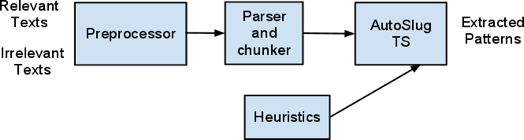
\includegraphics[scale=0.75]{workflow.png}

\subsubsection{Pattern Extraction in AutoSlog-TS}

We used a total of 13 heuristics for our system, 7 of these were for \texttt{Victim}, 4 were for \texttt{Target}, 2 were for \texttt{Perp\_Indiv} and 1 was for \texttt{Weapon}. There was one overlapping heuristic between \texttt{Victim} and \texttt{Target}. As we saw in the table in section 1.2, this resulted in a total of 99 unique patterns.

One particular challenge was that we had to modify the heuristics given in the paper[1] to suit our parser, first, because our it did not distinguish between active voice and passive voice, and second, because it did not identify syntactic roles (\textit{e.g.} subject, direct object, etc.) Of course, it is true that the dependency lists output by the parser could possibly be used to identify subjects and direct objects, but they were \textit{prima facie} not very accurate, so we decided not to use them.

\subsubsection{Pattern Matching in AutoSlog-TS}

This step occurs at runtime, after we've extracted patterns from the text. Our job at this point is basically to find patterns in a given text, rank the patterns that are most likely to contain correct predictions for a given slot, and then strip out the extraneous information we've extracted along with the embedded answer. The process is as follows:

\begin{enumerate}

\item \textbf{Preprocessing:} Splits the file into multiple texts and splits each text into meta text and main text. 

\item \textbf{Sentence-Splitting:} Splits the main text into different sentences using two patterns 1) dot followed by space or 2) dot followed by quotes.

\item \textbf{Pattern Matching:} Uses regular expressions to match the extracted patterns for victims, targets, and perpetrators in a given sentence. For our purposes, the forward patterns were the patters in which the relevant NP occured at the beginning (e.g ``\texttt{<NP> WAS\textbackslash s*[\textbackslash w]*\textbackslash s*MURDERED}"). In contrast, backward patterns are patterns in which the relevant NP occurs at the end (e.g. ``\texttt{MURDERED <NP>}” ). We looked for forward patterns first and then for backward patterns, if a forward pattern matched then the backward pattern containing the same verb is not considered. For example, if  ``\texttt{WAS\textbackslash s*[\textbackslash w]*\textbackslash s*MURDERED}" matched then we did not look for ``\texttt{MURDERED <NP>}".

\item \textbf{Parsing and NP Chunking:} If a sentence matches a particular pattern then we extract the relevant NP (i.e., for forward patterns we extract NP occurring just before the pattern and for backward patterns we extract the NP occurring after the pattern).

\end{enumerate}

A pictoral representation of this process is here:

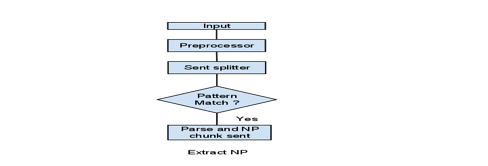
\includegraphics[scale=0.75]{patt.png}

\subsubsection{Post Proessing in AutoSlog-TS}

This module’s goal was to filter through the list of NPs returned by previous step before choosing the correct answers for each slot. We wrote methods that performed the following tasks in order to complete this module. 

\begin{enumerate}

\item \textbf{Extracting Multiple Answers from an NP:} We found that in some cases the extracted NP contained multiple answers separated by “and“, “accompanied by”, etc. We chose to look for such words and split the NP appropriately.

\item \textbf{Removing Synonyms:} We had a hard coded list of synonyms for this task. 

\item \textbf{Overlapping Answers Removal:} We often found that some of our answers overlapped (e.g., Hector Oqueli and Oqueli). In these cases, we simply chose the largest of the two strings.

\item \textbf{Appositive Removal:} Our answers for the victim slot usually contained appositives like ``Obama, President of the United States". So we maintained a list of relevant appositives and removed these if they were a part of the NP.

\item \textbf{Flag List:} We maintain flag list for all 3 of the slots. Flag list marks NPs that should be removed from consideration. For example, a victim flag list contained these words like \textit{headquarters} and \textit{embassy}. If such an NP in the list was reported, we simply removed it.

\item \textbf{Redundant word List:} This is a list of unnecessary words like verbs, weekdays, and prepositions that may be found alongside the answer, but which destroy the correctness of our answers.

\item \textbf{One word List:} This is a list of words which on their own could not be answers to any of the slots. Examples include words like \textit{headquarters}, \textit{urban}, \textit{salvador}, and so on. These words were summarily removed from any answers.

\end{enumerate}

\subsection{Predicting the \texttt{Weapon} Slot}

AutoSlog has the downside of being a very complicated slot with a number of different moving parts, and a significant pipeline, which makes it complicated to describe. In contrast, the \texttt{Weapon} slot is fairly simple: this is a weighted dictionary lookup. We find the weights using a cross-validated weight boosting scheme.

This is a viable approach because a very high percentage of the slots will accept an answer that is the \texttt{dev} set. Very close to all of the unique answers in the \texttt{test1} set are actually answers with more than one option, and almost always with at least one term we saw at least once in the \texttt{dev} set.

The question is how we know what the optimal weights are. The approach that made it into the final project works (roughly) as follows:

\begin{enumerate}
\item Begin with a hash table containing $key : value$ pairs, where $key$ is a word, and $value$ is an integer. Look at \texttt{dev} set's answer key, and set simply count the number of times you encounter any answer. Record this in the hash table.

\item Initialize a model. Run the model over some subset of the output (we did this using 2/3rds of the output). If the learner gets something wrong, weight that feature negatively. If it gets it right, weight that feature positively.

\item Do this repeatedly until you have some number of trainers, each trained on overlapping parts of the \texttt{dev} set.

\item Average their feature vectors; this gives you a weighted histogram.
\end{enumerate}

In the end, we simply hard-coded this weighted histogram into our submission. When it came time to predict the weapon, we adopted the following pipeline:

\begin{enumerate}
\item \textbf{Sentence-tokenize the document.}

\item \textbf{Look in the sentence for any of the words that were in the \texttt{dev} set answers.}

\item \textbf{Look in the histogram for the weight of each term found.}

\item \textbf{Output the term with the highest weight.}
\end{enumerate}


\section{Predicting the \texttt{Perp\_Org} Slot}

\texttt{Perp\_Org} is slightly more complicated than the \texttt{Weapon} slot, but the basic concept is similar. The difference is that, in the previous case, we used simple dictionary lookups for the weapons themselves. In this case, we supplemented this weighted histogram not just with the counts of the organization, but with the counts of the verbs around it. More concretely:

\begin{enumerate}
\item Look at the \texttt{dev} set answer key; build a hash table containing perp org answers paired with the count of the number of times they appeard (this is very similar to how we built the dictionary for the \texttt{Weapon} slot).

\item Now look at all the texts in the \texttt{dev} set. Sentence-tokenize each document, and then use NLTK's POS tagger to get POS annotations for every sentence. Pull all the verbs out and count how many times each occurrs in the same sentence as each particular word that was in the \texttt{dev} set answers. For example, if we have a word, \textit{bomb}, and the verbs that occur around it are \textit{explodes} and \textit{kills}, then we count them. At the end, we have a count of the words that occur next to bomb.
\end{enumerate}

We amplify the verb histogram using the algorithm described in the previous section. Then, using this histogram, we can construct the following algorithm:

\begin{enumerate}
\item \textbf{Sentence-tokenize the document.}

\item \textbf{Look in the sentence for any perp org that was also in the \texttt{dev} set.}

\item \textbf{If there exists at least one term, use NLTK's POS tagger to annotate that sentence; then pull all the verbs out. Look at the amplified counts of each verb, and sum them up.}

\item \textbf{Output the term that has the highest verb-weight sum.}
\end{enumerate}










\section{External resources}

Our final project uses NLTK and the Stanford Parser. However, we also at various points in the project used the Berkeley Parser, the Collins Parser, and the Stanford NER tagger, and both the lexicalized and normal Stanford PCFG parsers. NLTK was used for sentence and word tokenization, in addition to pos tagging and chunking.

\section{Contribution of each team member}

For a given slot, we ended up deploying the system that was most effective on the \texttt{test1} set. Although we performed many experiments, the \texttt{Victim}, \texttt{Perp\_Indiv}, and \texttt{Target} slots all ended up having an AutoSlog-TS backend, which was implemented almost entirely by \textbf{Vishay}. He was responsible for the pre- and post-processing of the AutoSlog system, as well as almost all of the internals. Finally, he implemented the initial \texttt{Incident} predictor, which was responsible largely for our score in the dry run.

The remaining slots were \texttt{Perp\_Org} and \texttt{Weapon}, both implemented by \textbf{Alex}. Additionally, Alex was responsible for integrating all the systems together, testing the holistic system, and tuning results of the holistic system. Further, Alex spent much of his time trying to produce viable alternatives to AutoSlog-TS, and although you won't see them in the final system, you can still see the code in the repository (especially if you sift through the commits in the .git file). This mainly served to inform the direction of the project: if it was the case that one of the systems outperformed AutoSlog-TS in one of the slots, it may have been the case that AutoSlog-TS would have been abandoned; it is by virtue of the fact that this didn't happen that we submitted the system we did. Additionally, outlines of the approaches in the presentation slides, and, to a lesser extent, in the ``originality" section.

\section{Emphasis / Originality}

Our final approach amounted mainly to a direct use of AutoSlog-TS, but what doesn't show up here is the stack of more creative schemes we implemented, but discarded. Some of these schemes were used on a limited bases---we talked about some of these (particularly secitons 1.3 and 1.4, when we talked about our approach to the \texttt{Weapon} and \texttt{Perp\_Org} slots. We would say that the boosted weighted historgram and parse-free organization identification schemes were probably the part of our final \textit{submitted} project that were most original.

Another thing that make our project relatively unique is the odd choice of technology we explored. We tried the Stanford parser, the Berkeley Parser, the Collins parser, and used more than a few components from the NLTK. While other groups were struggling for just good parses, we actually explored other options. Toward the end of the project we discovered that it was more effective to simply POS tag the sentences and chunk the NPs with the default NLTK chunker, which is a good example of how this is true. Another example is our weighted verb histogram scheme, which we used for \texttt{Perp\_Org} identification.

Lastly, we are unique in that we achieved reasonably good results on a number of methods; most groups picked one method alone and developed it until the deadline. Please see APPENDIX C for these results!

\section{Performance results and “glass box” analysis}

Our results follow:

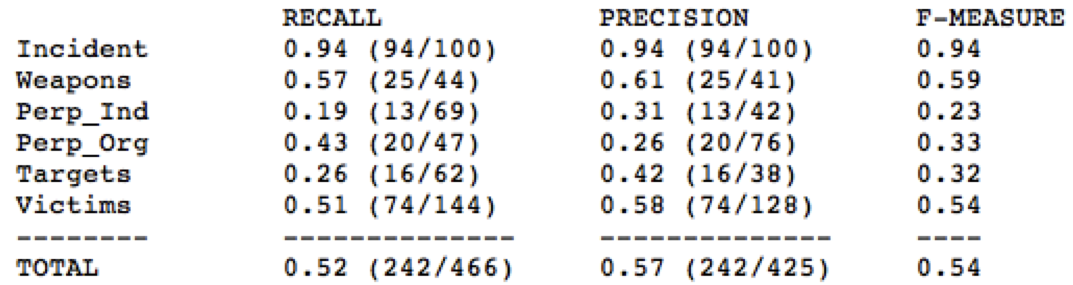
\includegraphics[scale=0.75]{result_t1.png} \\
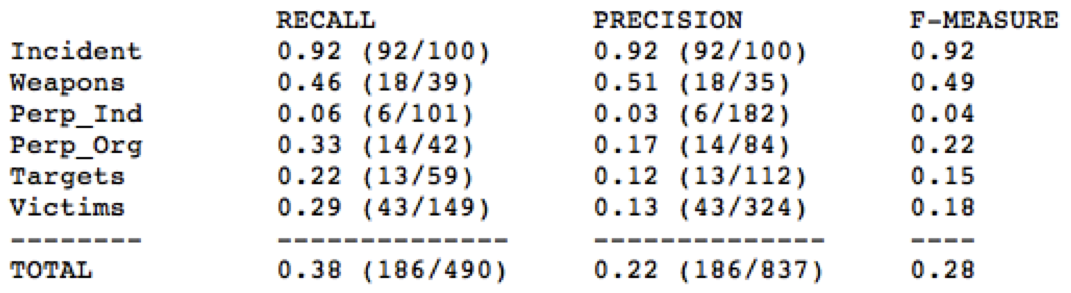
\includegraphics[scale=0.75]{result_t2.png} \\

As you can see, we do significantly better on the \texttt{test1} set than the \texttt{test2} set. There are a number of reasons for this, but the main one is that AutoSlog-TS's postprocessing step was created exclusively for, and exclusively using, \texttt{test1}'s data. This turns out to have caused the output to be very much overfitted, causing it to generalize poorly. Notice, for example, that the \texttt{Weapon} and \texttt{Incident} slots seem to have generalized quite nicely. Even the \texttt{Perp\_Org} does well compared to the rest of the slots.

What's really dragging down the average is the recall on \texttt{Perp\_Indiv}; when you just take out that one slot, it bumps our score by more than 4\%, from 0.28 to 0.32. This indicates that perhaps we're not doing as bad as it seems, \textit{prima facie}, because this is not even the worst slot---the worst slot by far is \texttt{Victim}, which produces 324 predictions for 149 slots. This is a consistent trend: in each of the AutoSlog-TS results (\texttt{Perp\_Ind}, \texttt{Targets}, and \texttt{Victims}), we make \textit{at least} twice as many predictions as there are actual answers. One simple modification we could do to improve our score would be to simply throttle the number of predictions we make in each slot, particularly the \texttt{Victim} slot. The effect of this is profound: consider if we had gotten a modest precision rate of 30\% (rather than the absurd 13\% we did get), we would have boosted our total score to 0.37. Obviously that is actually a pretty competetive result.

It's not hard to show convincingly that there are a number of fairly simple things that we could have done to increase our results \textit{without} affecting the actual learning algorithm. This is comforting to know, since it indicates that the things we learned during this project are not necessarily completely discounted by the abysmal performance on \texttt{test2}. While we did make at least one huge mistake, it is not true that our approach was completely hopeless.




\section{Surprise Factor}

\begin{enumerate}

\item Among 4 different parsers, we could barely get coherent output. To chunk NPs it was much more effective to word-tokenize, apply simple POS-tags using the default NLTK tagger, and then use NLTK's builtin NP chunker to find NPs.

\item We had not anticipated that the post processing module to be as complicated as it was. It was really difficult to sift through all the NPs extracted and get the correct answers.

\item Simple techniques worked better. Most people who had mined their answers from \texttt{dev} set did really well, even for general slots like \texttt{Victim}, \texttt{Target}, and \texttt{Perpet\_Indiv}.

\end{enumerate}

\section{Successes, regrets, and lessons learned}

Our success is straightforward: we were best-in-class on the \texttt{test1} set. This is undisputable. We also tried out a huge number of techniques and technologies, and were even successful in producing competetive results in other approaches that we tried.

That said, our results on the \texttt{test2} set were very bad, mainly because our post processing step was manually developed using only the \texttt{test2} data. This caused massive overfitting, and in retrospect, there are a number of different ways this could have been avoided:

\begin{enumerate}

\item Building the system on the \texttt{dev} set alone, and using the test set \textit{only} for tuning.
\item Building an ML-based post processor.
\item Using an NER tagger plus a dictionary (for nameless victimsm \textit{e.g.}, people, child, wife, etc.) to validate the answers for the victim slot.

\end{enumerate}


This is a big lesson not really because we didn't know about overfitting before (we did), but because it makes the lesson of overfitting \textit{very} concrete: avoid anything that even \textit{looks} like overfitting.













\section*{APPENDIX A}

This appendix lists all the heuristics we used along with regex patterns.  
All of these Heuristics were taken from the AutoSlog-TS publication.

\begin{verbatim}
Slot 	  Heuristic 	         Regex 
victim 	NP VBD VBN           	(\[[^/]*?\])\/NP\s+(\w+?)\/VBD\s+(\w+?)\/VBN
victim  NP VBD NN             (\[[^/]*?\])\/NP\s+(\w+?)\/VBD\s+(\[.*?\])\/NP\s+
victim  VBD NP                \s+(\w+?)\/VBD\s+(\[[^/]*?\])\/NP
victim  VB(all) TO VB NP      \s+(\w+?)\/VB\w{0,1}\s+(\w+?)\/TO\s+(\w+?)\/VB\s+(\[[^/]*?\])\/NP
victim  VBG NP                \s+(\w+?)\/VBG\s+(\[[^/]*?\])\/NP
victim  NN VBD NP	            (\[[^/]*?\])\/NP\s+(\w+?)\/VBD\s+(\[[^/]*?\])\/NP
victim  NN IN NP	             (\[[^/]+?\])\/NP\s+(\w+?)\/IN\s+(\[[^/]*?\])\/NP
Perp_I  NP VB(all)	           (\[[^/]*?\])\/NP\s+(\w+?)\/VB\w{0,1}
Perp_I  NP VBD TO VB          (\[[^/]*?\])\/NP\s+(\w+?)\/VBD\s+(\w+?)\/TO\s+(\w+?)\/VB
Weapon  VB IN NP              \s+(\w+?)\/VB\w{0,1}\s+(\w+?)\/IN\s+(\[[^/]*?\])\/NP
Target  VB(all) TO VB NP      \s+(\w+?)\/VB\w{0,1}\s+(\w+?)\/TO\s+(\w+?)\/VB\s+(\[[^/]*?\])\/NP
Target  VBD NP	               \s+(\w+?)\/VB\w{0,1}\s+(\[[^/]*?\])\/NP
Target  NN IN NP              (\[[^/]+?\])\/NP\s+(\w+?)\/IN\s+(\[[^/]*?\])\/NP
Target  VBD VB(all) prep NP   \s+(\w+?)\/VBD\s+(\w+?)\/VB\w{0,1}\s+(\w+?)\/IN\s+(\[[^/]*?\])\/NP
\end{verbatim}

 



\section*{APPENDIX B}

This Appendix Contains all the patterns we used for Extraction System. Most of these patterns were learnt using the AutoSlog-TS, and some of them were added( or modified ) manually.


\begin{verbatim}
VICTIM

<NP> DIED INSTANTANEOUSLY
<NP> WAS\s*[\w]*\s*ASSASSINATED
<NP> WAS\s*[\w]*\s*INJURED
<NP> WAS\s*[\w]*\s*KIDNAPPED
<NP> WAS\s*[\w]*\s*KILLED
<NP> WAS\s*[\w]*\s*MURDERED
<NP> WAS\s*[\w]*\s*WOUNDED
<NP> WERE\s*[\w]*\s*KILLED
<NP> WERE\s*[\w]*\s*KIDNAPPED 
<NP> WERE\s*[\w]*\s*ABDUCTED 
<NP> WERE\s*[\w]*\s*ASSASINATED
<NP> WERE\s*[\w]*\s*INJURED 
<NP> WERE\s*[\w]*\s*MURDERED
<NP> WERE\s*[\w]*\s*WOUNDED
<NP> WERE\s*[\w]*\s*SHOT
<NP> WAS\s*[\w]*\s*SHOT
ASSASSINATION OF  <NP>
ASSASSINATIONS OF  <NP>
ASSASSINS OF  <NP>
ATTACK ON  <NP>
ATTACKED  <NP>
BLOOD OF  <NP>
BODIES OF  <NP>
BURIAL OF  <NP>
DEATH OF   <NP>
DEATHS OF <NP>
DISAPPEARANCE OF <NP>
ELIMINATED <NP>
FUNERAL OF <NP>
FUNERALS OF <NP>
KIDNAPPED <NP>
KIDNAPPING OF <NP>
KIDNAPPINGS OF <NP>
KILLED <NP>
KILLING <NP>
KILLING OF <NP>
LIVES OF <NP>
LOSS OF <NP>
MACHINEGUNNED <NP>
MASSACRE OF <NP>
MURDER OF <NP>
MURDERED <NP>
MURDERERS OF <NP>
MURDERS OF <NP>
WOUNDED  <NP>
\end{verbatim}

\begin{verbatim}
PERP_INDIV

<NP>  ASSASSINATED
<NP> ATTACKED
<NP>BLEW
<NP> BOMBED
<NP>  BURNED
<NP> COMMITTED
<NP> DETONATED
<NP> FIGHTERS
<NP>  FIRED
<NP>  HURLED
<NP>  INFLICTED
<NP>  KIDNAPPED
<NP>  KILLED
<NP>  MACHINEGUNNED
<NP>  SABOTAGED
WAS KIDNAPPED BY <NP>
WERE KIDNAPPED BY <NP>
WERE ABDUCTED BY <NP>
WAS ABDUCTED BY <NP>
WAS ATTACKED BY <NP>
WAS KILLED BY <NP>
WERE KILLED BY <NP>
WAS MURDERED BY <NP>
WERE MURDERED BY <NP>
WAS SHOT BY <NP>
WERE SHOT BY <NP>
WAS ASSASSINATED BY <NP>
WERE ASSASSINATED BY <NP>
WAS INJURED BY <NP>
WERE INJURED BY <NP>
WERE WOUNDED BY <NP>
WAS WOUNDED BY <NP>
WERE DETONATED BY <NP>
\end{verbatim}

\begin{verbatim}
TARGET

AN ATTACK ON <NP>
ATTACK ON <NP>
ATTACKED <NP>
ATTACKS ON <NP>
BOMBED <NP>
BOMB ATTACK ON <NP>
BOMB IN <NP>
BOMBING <NP>
BURNED <NP>
BURNING <NP>
DAMAGED <NP>
DESTROYED <NP>
DESTRUCTION OF <NP>
DOWNED <NP>
DOWNING OF <NP>
DYNAMITE ATTACK ON <NP>
FIRED <NP>
HIT <NP>
MACHINEGUNNED <NP>
SABOTAGED <NP>
SET FIRE TO <NP>
\end{verbatim}



Perp\_Org   ( We got these patterns while reviewing the other slots. we did not get time to implement these)

\begin{verbatim}
GUERRILLAS OF
MEMBERS OF
ACTIVE MEMBER OF
SPOKESMAN OF 	
\end{verbatim}

\section{APPENDIX C}

When we ran the approach we used on \texttt{Weapon} over all the slots except \texttt{Incident}, we got the following results:

\texttt{dev}
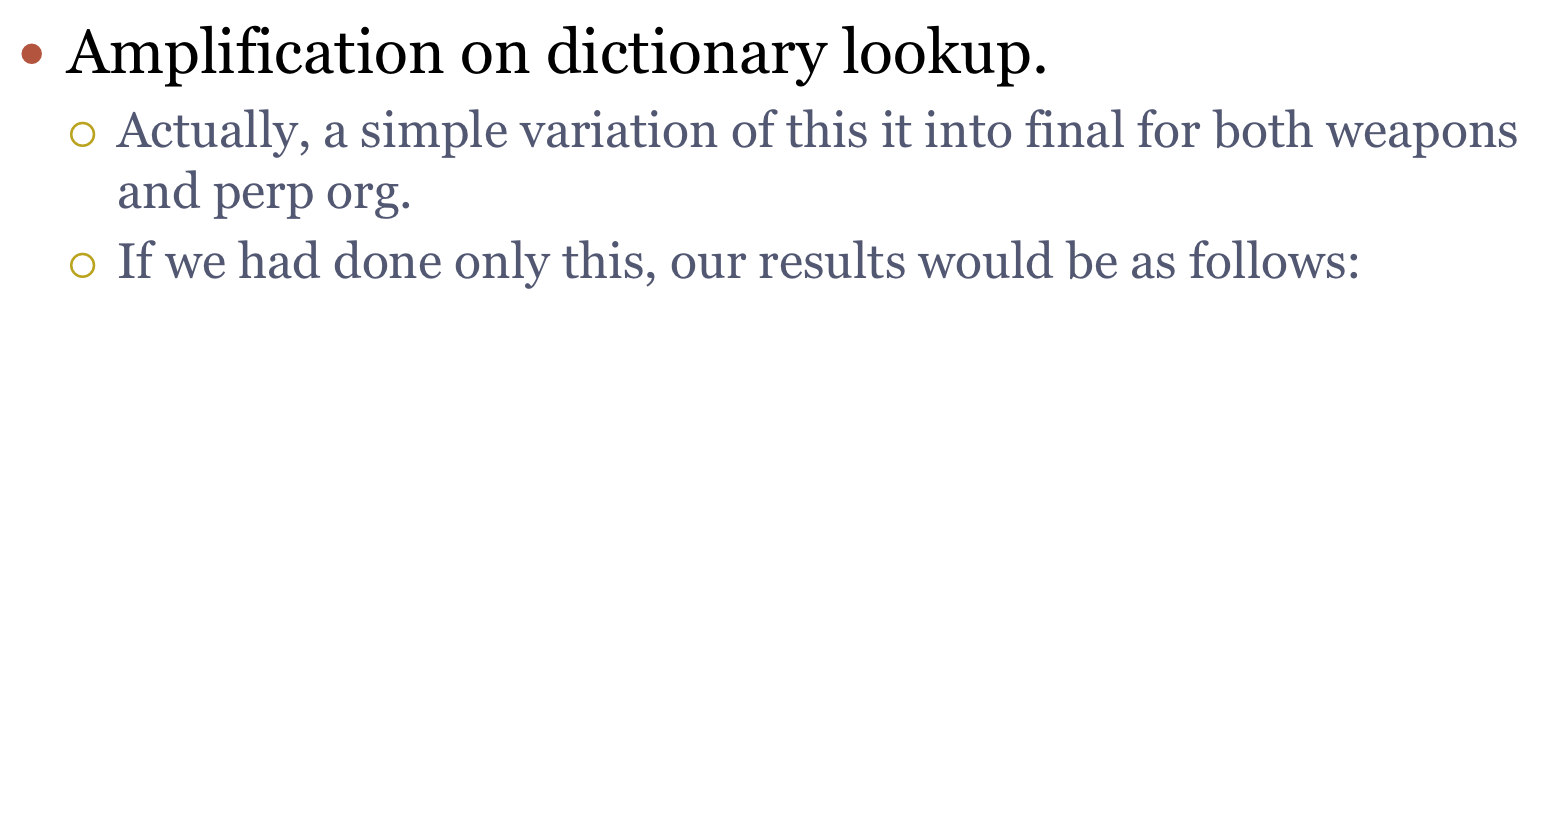
\includegraphics[scale=0.75]{amp_dev.png} \\

\texttt{test1}
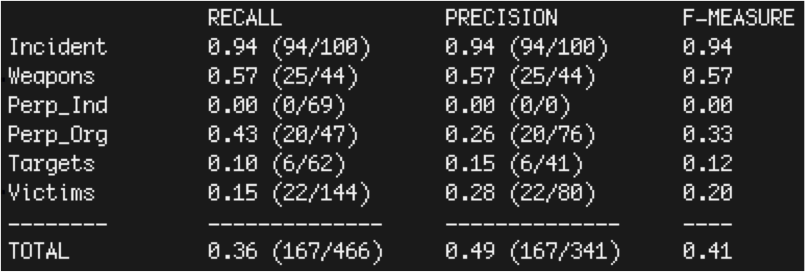
\includegraphics[scale=0.75]{amp_t1.png} \\

\texttt{test2}
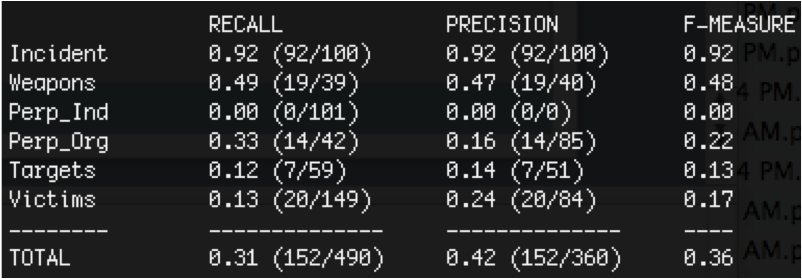
\includegraphics[scale=0.75]{amp_t2.png} \\

When we ran a slightly modified version of approach we used on \texttt{Perp\_Org} over all the slots except \texttt{Incident}, we got the following results (note the actual perp org slot is slightly different):



Finally, combining both of them, we get the following:

\texttt{dev}
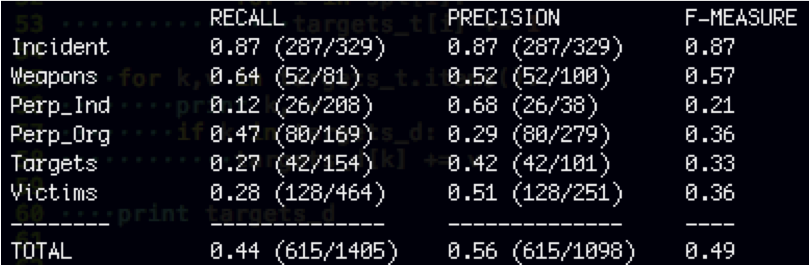
\includegraphics[scale=0.75]{amphist_dev.png} \\

\texttt{test1}
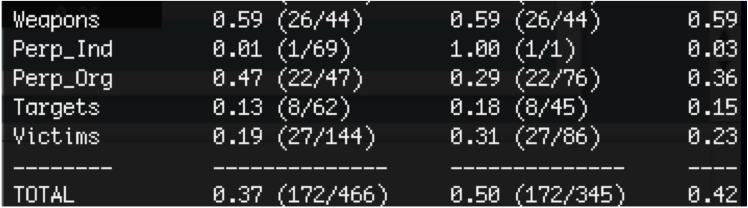
\includegraphics[scale=0.75]{amphist_t1.png} \\

\texttt{test2}
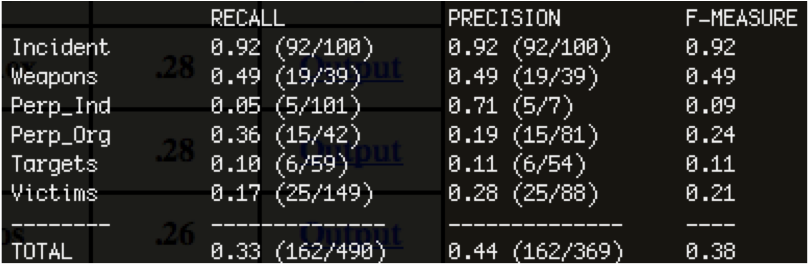
\includegraphics[scale=0.75]{amphist_t2.png} \\


\end{document}